\documentclass[12pt]{article}

\usepackage{sbc-template}

\usepackage{graphicx,url,wrapfig,lipsum}

%\usepackage[brazil]{babel}   
%\usepackage[latin1]{inputenc}  
\usepackage[utf8]{inputenc}		% Codificacao do documento (convers\~{a}o autom\'{a}tica dos acentos)
\usepackage{color}

\usepackage{verbatimbox}
\usepackage{framed}
\usepackage{listings}
\usepackage{adjustbox}
\usepackage{pdfpages}

\usepackage{framed}
\usepackage{adjustbox}
\usepackage{listings}
\definecolor{codegreen}{rgb}{0,0.6,0}
\definecolor{codegray}{rgb}{0.5,0.5,0.5}
\definecolor{codepurple}{rgb}{0.58,0,0.82}
\definecolor{backcolour}{rgb}{0.95,0.95,0.92}

% MUDAR NO PRINCIPAL
\lstset{basicstyle=\fontsize{8}{10}\ttfamily, numbers=left, numberstyle=\tiny\color{black}, stepnumber=1, numbersep=8pt, tabsize=3, showspaces=false, showstringspaces=false, frame=single, breaklines=true, moredelim=**[is][\color{codegreen}]{@}{@},moredelim=**[is][\color{red}]{|}{|},moredelim=*[is][\color{codepurple}]{/*}{*/},moredelim=*[is][\color{blue}]{@*}{*@}}

%%% MERGE COM PRINCIPAL     
\definecolor{maroon}{rgb}{0.5,0,0}
\definecolor{darkgreen}{rgb}{0,0.5,0}

 %%% MERGE COM PRINCIPAL     
 
\sloppy

\title{Brazil's IXP requirements, limitations and security issues: a survey}

\author{Humberto Silva Galiza de Freitas\inst{1}, Christian Esteve Rothenberg\inst{2}, Jeronimo Aguiar Bezerra\inst{3}}

\address{Rede Nacional de Ensino e Pesquisa (RNP) \\
		Diretoria de Engenharia e Operações (DEO)\\
		Núcleo de Engenharia de Redes de AmLight (NEG AmLight)\\
  Campinas -- SP -- Brasil
\nextinstitute
  Universidade Estadual de Campinas (UNICAMP)\\
  Faculdade de Engenharia Elétrica e de Computação (FEEC)\\
  Information \& Networking Technologies Research \& Innovation Group (INTRIG)\\
  Campinas -- SP -- Brasil
  \nextinstitute
  Florida International University (FIU)\\
  Center for Internet Augmented Research and Assessment (CIARA)\\
  Miami -- FL -- USA
  \email{humberto.galiza@rnp.br, christian@unicamp.br, jbezerra@fiu.edu}
}

\begin{document} 

\maketitle

\begin{abstract}
lorem ipsum lorem ipsum lorem ipsum lorem ipsum lorem ipsum lorem ipsum lorem ipsum lorem ipsum lorem ipsum lorem ipsum lorem ipsum lorem ipsum lorem ipsum lorem ipsum lorem ipsum lorem ipsum lorem ipsum lorem ipsum lorem ipsum lorem ipsum lorem ipsum lorem ipsum lorem ipsum lorem ipsum lorem ipsum lorem ipsum lorem ipsum lorem ipsum lorem ipsum lorem ipsum lorem ipsum lorem ipsum lorem ipsum lorem ipsum lorem ipsum lorem ipsum lorem ipsum lorem ipsum lorem ipsum lorem ipsum lorem ipsum lorem ipsum lorem ipsum lorem ipsum lorem ipsum lorem ipsum lorem ipsum lorem ipsum lorem ipsum lorem ipsum lorem ipsum lorem ipsum lorem ipsum lorem ipsum lorem ipsum lorem ipsum lorem ipsum lorem ipsum lorem ipsum lorem ipsum.

\end{abstract}

\section{Introduction}

Internet eXchange Points (IXP) are the natural successors of the four Network Access Points (NAP) responsible for interconnecting different networks in the early stages of today's Internet. The benefits achieved regarding performance and security are the main reason for the key role that the IXPs plays in the present Internet ecosystem~\cite{norton20142014}.

Although the dynamics of operation, criticality, and security aspects of an IXP are well-known and quite often under discussion by the network operators community, only recently the scientific community began to delve into this subject. In this sense, the work of~\cite{ager2012anatomy} pioneered with the flow analysis from a large European IXP. The authors concluded, among other things, that the traffic volume exchanged between the IXP members was analogous to levels observed in a Tier-1 Internet Service Provider (ISP) network. 

In the same context in Brazil, the work of~\cite{brito2015anatomia} innovated by bringing for the first time an analysis of the IXP ecosystem in operation in the country. The authors compiled valuable information about the characterization of the types of members present in these environments and their connectivity graphs at the Autonomous System (AS) level, being able to determine the peering potential in each IXP. 

From an operational perspective, despite the fact that the Federal Interconnection eXchange Point (FIX) is considered the first public IXP in Brazil~\cite{fix2002}, the PTTMetro project launched in 2004 and coordinated by the Brazilian Regional Internet Registry Authority (NIC.BR) was, in fact, the responsible for the spreading of regional commercial IXPs in Brazil. Since then, the project has expanded the number of IXPs and the Points of Presence (PoPs) under its management across the country, and thus contributed to the development and improvement of national quality Internet. More recently, the project was renamed to IX.BR, and is currently operating in 24 cities in Brazil, exchanging near 2 Tbps of aggregated traffic~\cite{pttmetro}, being considered the 4th biggest in the world based on the number of members~\cite{putta2016region}.

Notwithstanding the clear benefits and advances brought about by large-scale deployment of IXPs in Brazil, the current model poses several problems, in the vast majority derived from its own architecture. These issues might end up affecting at different levels its  security, scalability, and resiliency. The occurrence of network events or security incidents can compromise all or part of its operation, creating damages to its image and mission. In these cases, insecurity and instability set up in the routing environment contribute to the increase in distrust among the participants, as well as distancing possible new members.

The main contribution of the present work is to bring a Survey of the technical requirements and weaknesses of public IXPs in Brazil, presenting a non-exhaustive list of top security and limitations issues that affect these requirements. Despite the focus on Brazil, this study may contribute to a better understanding about the limitations and improvements that can be adopted in other IXPs using  similar models. For each of the identified problems, possible solutions that follows the IXP model assumptions and operations guidelines and also that keeps IXP's stability, availability and scalability are provided. 

Moreover, as some of the presented problems can not be addressed due to limitations in the current Ethernet/IP architecture, this paper also contributes in assessing the feasibility of adoption of some concepts from Software-Defined Networking (SDN) and OpenFlow protocol~\cite{specification2009version} to address these deficiencies. The employment of such concepts can be the first step in the transformation of the current IXP model into a lightweight version of Software-Defined Internet eXchange (SDX) concept~\cite{gupta2015sdx}.

The rest of this paper is structured as follows. Section~\ref{sec:background} provides an overview about IXP's concepts, architecture and operations activities. Section~\ref{sec:analysis} dissects the current architectural problems and limitations using a bottom-up approach. Following, Section~\ref{sec:ongoingresearch}, discusses some ongoing research efforts that address the issues raised, including the application of SDN and OpenFlow concepts. We conclude our work and discuss future directions in Section~\ref{sec:conclusion}.

%Apesar dos nítidos benefícios e avanços trazidos pela implantação em larga escala de IXPs pelo Brasil, o modelo atual de operação carrega diversos problemas, muitos dos quais derivados da sua própria arquitetura. Esses problemas acabam afetando em diferentes níveis o seu gerenciamento, segurança, escalabilidade, resiliência e gestão. A ocorrência de incidentes de rede ou segurança em um IXP pode comprometer toda ou parte da sua operação, gerando riscos à sua imagem e missão. Nestes casos, a insegurança e instabilidade criadas no ambiente de roteamento contribui para o aumento na desconfiança entre os participantes, e bem como para o distanciamento de novos possíveis membros participantes.

%A contribuição deste trabalho é trazer um Survey dos requisitos e limitações técnicas dos IXPs públicos no Brasil, elencando uma lista não exaustiva dos principais problemas de segurança que atingem esses requisitos. Apesar do foco no Brasil, esse estudo pode contribuir para um melhor entendimento das limitações e melhorias que podem ser adotadas em outros IXPs com modelos similares. Para cada um dos problemas apontados serão catalogadas possíveis soluções com foco na estabilidade e escalabilidade do IXP, obedecendo as premissas que norteiam seu funcionamento. Por fim, serão avaliados os benefícios da adoção dos conceitos das Redes Definidas por Software, tornando os IXPs em Ponto de Troca de Tráfego Definidos por Software, do inglês \textit{Software-Defined Internet eXchange} (SDX), na resolução de alguns dos problemas bem conhecidos na arquitetura tradicional de troca de tráfego.

%Este artigo está organizado da seguinte forma: na Seção~\ref{sec:background} serão introduzidos os conceitos e arquitetura de funcionamento de um IXP. Na Seção~\ref{sec:analise} serão dissecados os problemas que atingem as camadas que formam a operação de um IXP. Em seguida, na Seção~\ref{sec:trabrelacionados} serão catalogados alguns trabalhos relacionados que endereçam as questões apontadas, além de uma breve introdução do conceito de SDX. Por fim, na Seção~\ref{sec:conclusion} serão feitas algumas considerações finais e sugestões de direcionamentos futuros.

%Internet eXchange Points are the heart of today's Internet. In Brazil, the roll out of IXPMetro project in 200x have contributed to develop Brazil's Internet as well as to improve it's quality. On the other hand, many problems affect the current model, not only in Brazil but over the world, since most IXPs use pretty much the same Ethernet based model today.

%Software-Defined Networking is a new networking approach that promises, among other things, turn the networks more smart by decoupling the control plane from the data plane, as well as adding programmability support to the network. OpenFlow is the most famous protocol in this novel, and was created as a joint effort of many different networking organizations, to provide all the SDN abstractions.

%These are trend topics today and have a good relevance to the academia. Understanding how SDN/OpenFlow could bring benefits to a real world use case will bring new challenges, but the most important achievement of this research will be delivering a true scalable model, with support to more refined Traffic Engineering capabilities and improved security.

%This work presents the challenges affecting the current Internet eXchange Point (IXP) model used in Brazil, identifying and evaluating the impact of its principal weakness in the scope of security, scalability, resiliency and operations. As a response to these challenges, a new design, based on the novel Software-Defined Networking approach, will be proposed and is expected that this new model could be able to address the primary concerns affecting the current model, adding more capabilities to it, while keeping the original foundations that drives the IXP operation.

%Though the critical importance that IXPs represent to the Internet, as could be easily verified in the literature, its \textit{modus operandi} carries several problems affecting at different levels its security, scalability, resiliency and management. These issues can compromise all or part of its operation, damaging its image and mission, due to the insecurity and instability created in the traffic routing environment, generating mistrust to the current members, as well as distancing possible new associates.

%In this work, some of the principal issues affecting the current model of traffic exchange in Brazil are outlined. 

\section{Background}
\label{sec:background}
Prior to its worldwide deployment and coverage, the Internet routing was centralized at four NAPs located in the U.S. These NAPs were public exchange facilities where commercial ISPs got interconnected to exchange traffic. As part of the NSFNET transition strategy to the modern Internet, these centralized access points were replaced by distributed IXPs. Currently, they are present in a number of countries, playing a key role in the Internet ecosystem by carrying out a large amount of traffic~\cite{chatzis2013importance}. 

From a design point of view, while the traditional IXPs can be classified into Layer-2 and Layer-3 IXPs, the prevalent model nowadays is the Layer-2 shared medium, like Ethernet, on top of which the IXP services are offered. This choice is due to the simplistic design requirements when providing a Layer-2 topology, as well as the easy and reduced costs for growing the switching fabric when compared to a Layer-3 solution.

As already mentioned, the simplest IXP design includes a Layer-2 pure switch, where the IXP connectors exchange traffic. However, as depicted in Figure~\ref{fig:ixparch1}, to scale this design and assure resiliency in the architecture, more switches may be added to the Layer-2 topology creating a switching fabric. In the same sense, the IXP can expand its own operations to cover a wide area (e.g., a metropolitan region). In this case, besides having multiple switches, the IXP can have multiple PoPs under the same Layer-2 shared medium, where all PoPs are interconnected, creating a full-mesh, or simply a distributed switching fabric.

\begin{figure}
\centering
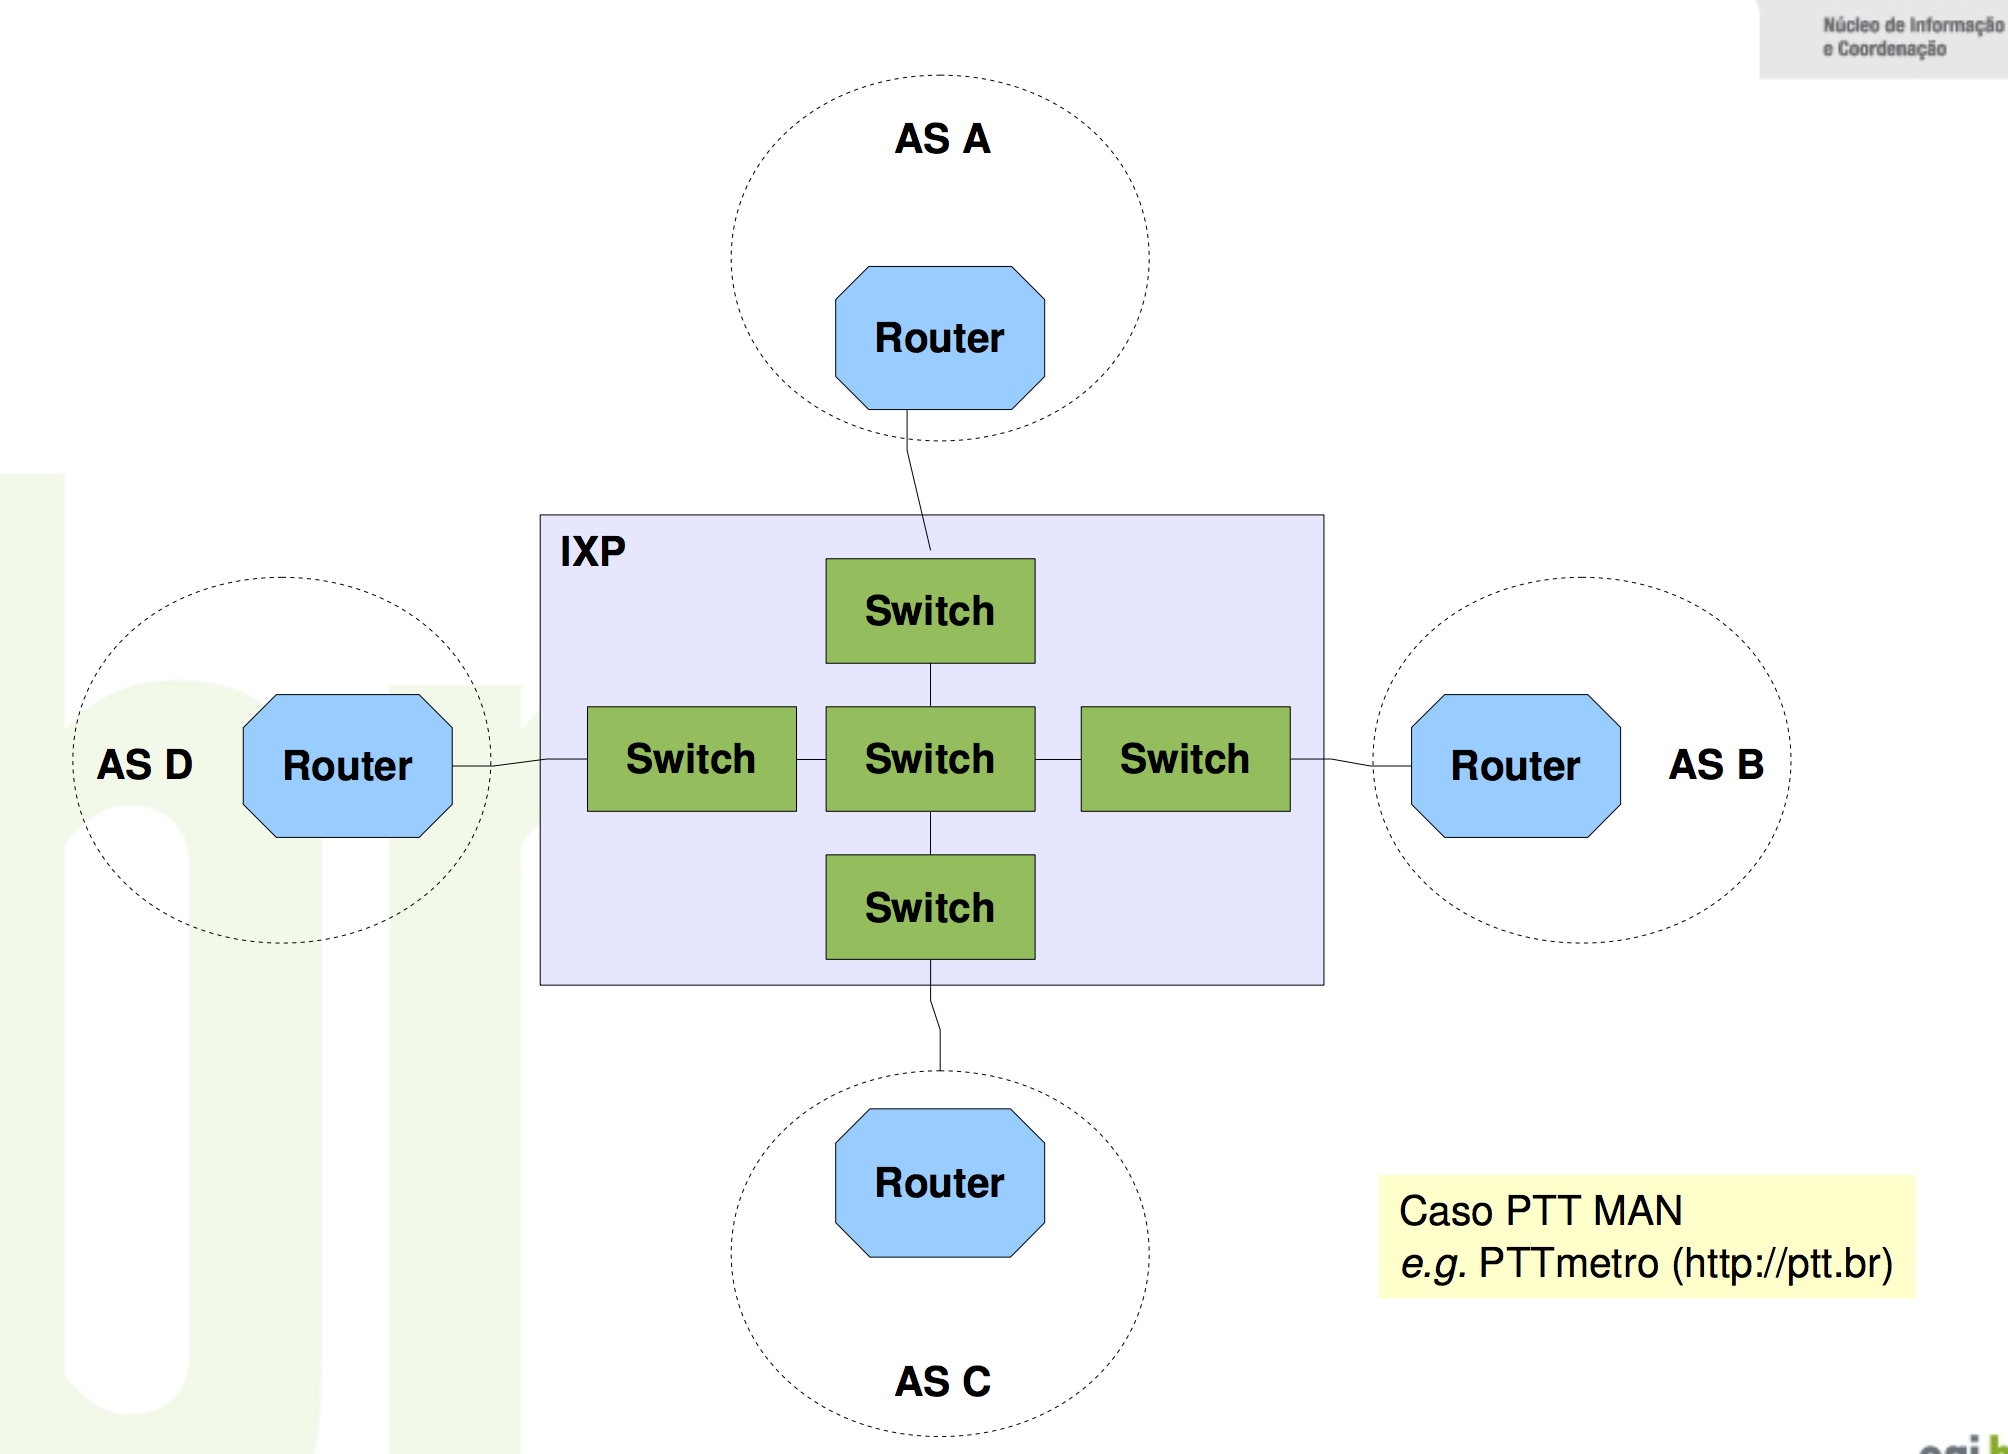
\includegraphics[scale=0.25]{imagens/ptt-fabric.png} 
\caption{IXP traditional architecture with multiple PoPs. CHANGE PICTURE!!}
\label{fig:ixparch1}
\end{figure}

In general, most IXPs in operation nowadays adopt a technical model where the switching fabric is essentially an enormous flat Ethernet domain, based on different technologies such as IEEE Std 802.1q Medium Access Control (MAC) Bridges, Virtual Bridge Local Area Networks (VLANs) and Virtual Private Lan Service (VPLS)~\cite{rfc4761,rfc4762}. On top of such (distributed) switching fabric, the members are free to set up peering agreements (BGP sessions) with other as they wish to exchange routes.

This method of peering at IXPs were very common in the early stages of IXPs deployment. However, it became a tough operational problem managing a large number of bilateral BGP sessions when the number of IXP members and peering agreements grew. In response to this challenge, the route-servers emerged as a method of interconnecting BGP speaking routers using a third-party system~\cite{rfc7947}. 

\begin{figure}
\centering
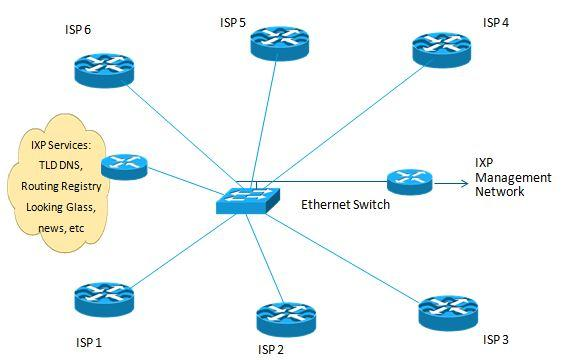
\includegraphics[scale=0.2]{imagens/route-server.jpg} 
\caption{IXP route-server in operation. CHANGE PICTURE!!}
\label{fig:routeserver}
\end{figure}

In this context, each IXP member set up one or more BGP sessions with the route-server and it, in turn, forwards the route information to each route-server client connected. This method of peering is also known as Multilateral peering, and Figure~\ref{fig:routeserver} illustrates the dynamic of its operation. In fact, the route-server operation is very similar to the route-reflector as specified in~\cite{rfc4456}, except that it operates over an eBGP session instead of internal BGP (iBGP).

Besides the bilateral and multilateral peering arrangements, additional services may be offered, or even, sold using the peering fabric. A common "package" often seen in different IXPs around the globe, includes, but do not limit to, DNS TLD service, NTP service, Internet Routing Registry (IRR) service, and Looking Glass. Usually these services are offered and maintened by the IXP operator.

In addition to this set of services, IXP members are allowed to buy/sell IP Transit from/to its partners. This can be achieved very straightforward by setting up a bilateral transit BGP session over the shared VLAN, or by asking the IXP operator to set up a dedicated VLAN between the two members, and then, setting up the transit BGP session. While this practice contrast with the IXP itself definition, in fact, it is a very common practice nowadays due to the easy of deployment, and the possibility of making business with a wide variety of members, in contrast with purchasing or selling IP transit from/to a dedicated partner. 

Brazil's IX.BR project adopted the european IX model~\cite{euroix2012}, i.e, the peering fabric is operated by a not-for-profit independent organization, usually NIC.BR and the Brazilian Research and Education Network (RNP), and the fabric may be spread across potentially many competing colocation facilities. Thus, the IX.BR members can choose the facility that best meets their needs. For instance, São Paulo's city IXP is the biggest one in operation, with around 500 connectors, exchanging near 1.5Tbps of traffic daily. Figure~\ref{fig:pttsp} illustrates São Paulo's city IXP PoPs interconnection in a live traffic map.
\begin{figure}
\centering
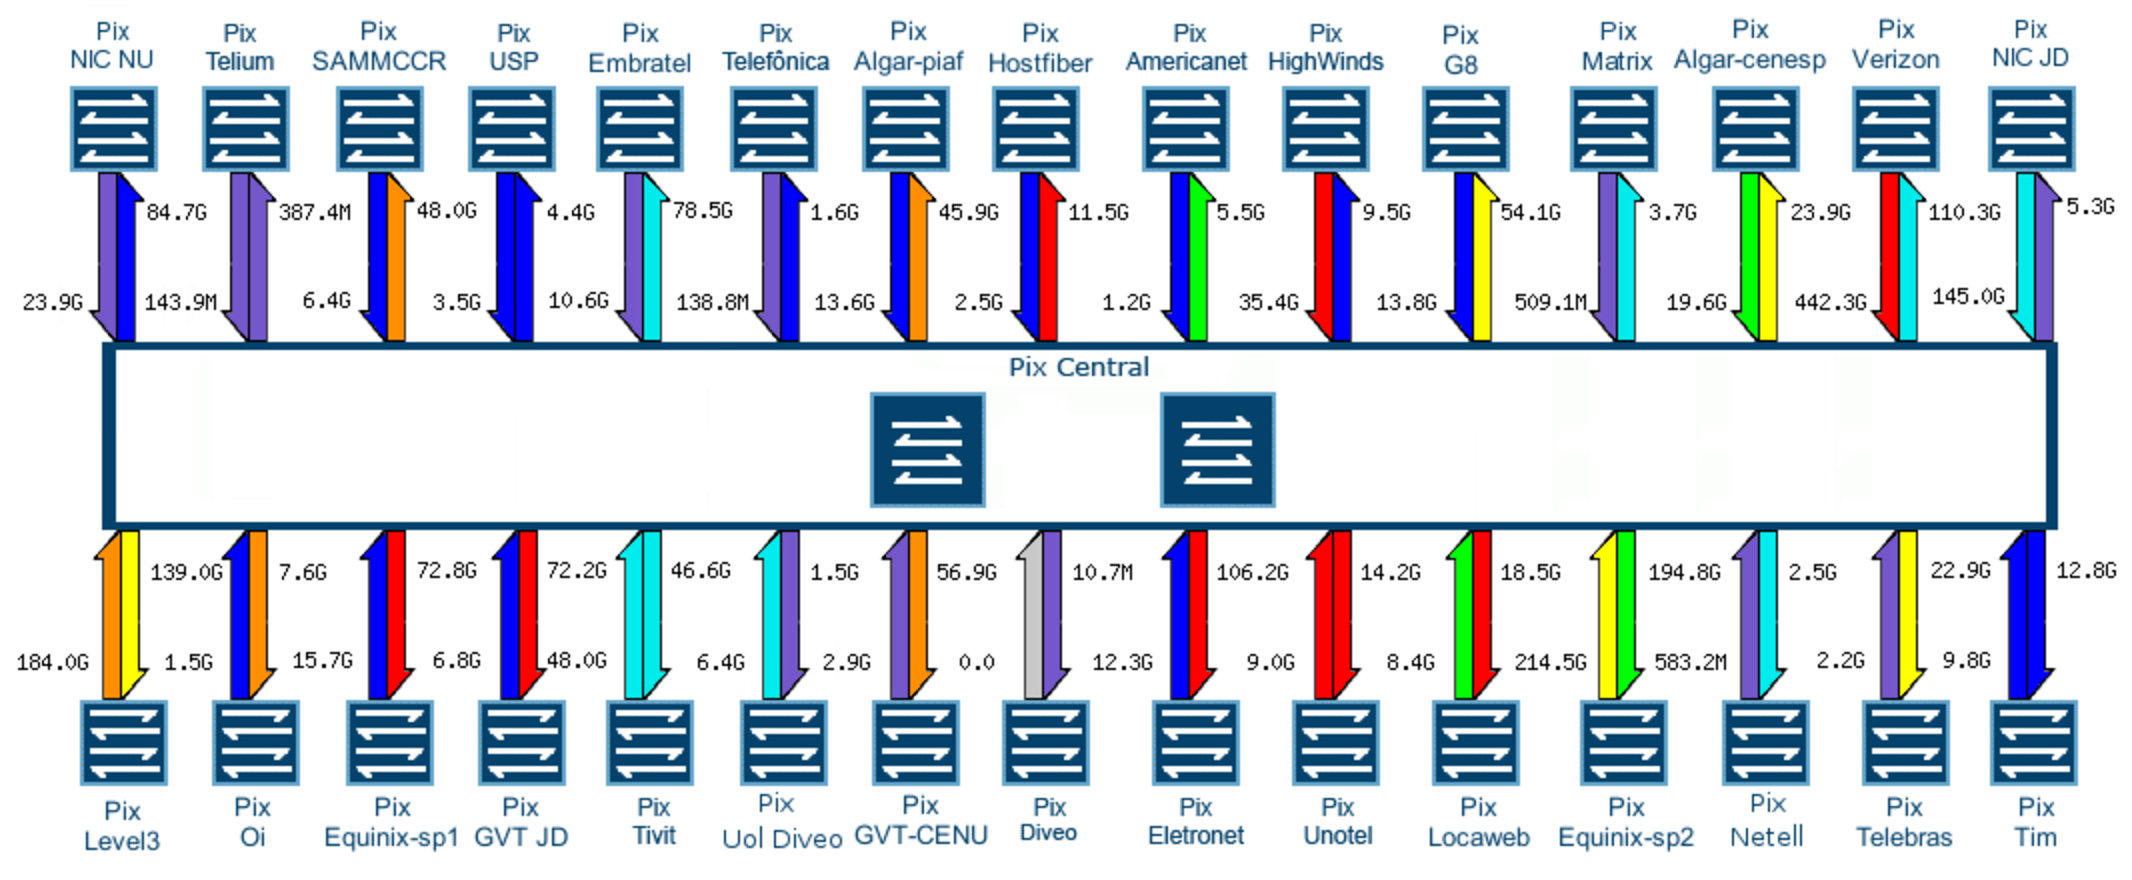
\includegraphics[scale=0.4]{imagens/ptt-sp} 
\caption{São Paulo's IXP links between colocation facilities (PoPs).}
\label{fig:pttsp}
\end{figure}

%Em geral, a maioria dos IXPs em operação hoje adotam um modelo em que a matriz de comutação de tráfego é essencialmente um grande domínio~\textit{ethernet} baseado em diferentes tecnologias, como as Redes Locais Virtuais, do inglês \textit{Virtual Area Networks} (VLANs) baseadas no padrão IEEE Std 802.1q e o Serviço Privado de Lan Virtual, do inglês \textit{Virtual Private Lan Service} (VPLS)~\cite{rfc4761} e ~\cite{rfc4762}. Em cima dessa matriz de comutação os participantes do IXP criam sessões BGP para trocar rotas.

%In general, most of the IXPs in operation today adopt a model where the switching fabric is essentially an enormous flat ethernet domain, based on different technologies such as IEEE Std 802.1q Medium Access Control (MAC) Bridges and Virtual Bridge Local Area Networks and Virtual Private Lan Service (VPLS). On top of such switching fabric, all members set up BGP sessions to exchange routes.

%\subsection{Multilateral Peering Agreement}
%Acordo de Troca de Tráfego Multilateral (ATM): permite a troca de tráfego com todas as redes participantes do IXP;
%\subsection{Bilateral Peering Agreement}
%Acordos Bilaterais: permite a troca de tráfego com participantes específicos;
%\subsection{Buying and Selling IP Transit}
%Compra e venda de trânsito: permite o acesso a outras redes através de participantes do IXP que ofereçam esta possibilidade.
%\subsection{Operations and Management of an IXP}

\section{Issues and Limitations: Bottom-up Analysis}
\label{sec:analysis}
Despite of the success of the IXP model, and particularly in Brazil, the country-wide IXP deployment benefits, there are problems and limitations imposed by the architecture and technologies is use. 

Introduzir os problemas que afetam o modelo atual...
\subsection{Infrastructure}
\label{sec:infraestrutura}

\subsection{Control Plane}
\label{subsec:issues_cp}
Introduzir os problemas que afetam o plano de controle

\subsubsection{\textit{Broadcast Storming} na Matriz de Comutação}
\label{subsubsec:broadcast_storm}

As redes de computadores puramente em camada-2 são bem conhecidas por terem problemas de escalabilidade. Ao passo que o tamanho do domínio de \textit{broadcast} aumenta, o nível de tráfego de \textit{broadcast} de protocolos como o \textit{Address Resolution Protocol} (ARP) aumenta. Quantidades significativas de tráfego de \textit{broadcast} constituem uma carga particular para a rede, porque todos os dispositivos desse domínio devem processar e, eventualmente, atuar sobre esse tráfego. 

As fontes de \textit{broadcast storming} na matriz de comutação incluem, mas não se limitam a: (1) implementações fracas de protocolos de detecção e prevenção de \textit{loops} na camada 2; (2) erros de configuração por parte dos participantes do IXP. Em casos extremos, essa enxurrada de tráfego \textit{broadcast} podem atingir um nível capaz de reduzir em parte ou no todo a capacidade operacional de uma rede~\cite{rfc6820}.

%However, flat Layer-2 networks have long been known to have scaling problems. As the size of a broadcast domain increases, the level of broadcast traffic from protocols like Address Resolution Protocol (ARP) increases. Significant amounts of broadcast traffic pose a particular burden on the network because every device in such domain must process and possibly act on such traffic. Sources of broadcast storms in the switching fabric include, but does not limit to: (1) poor implementations of loop detection and prevention protocols; (2) IXP members misconfiguration errors. In extreme cases, these storms can occur where the quantity of broadcast traffic reaches a level that actually brings down part or all of a network~\cite{rfc6820}. 

Apesar de o senso comum ao projetar redes de \textit{data center} seja dividir grandes domínios de transmissão em múltiplos segmentos de rede, tal solução não é aplicável a um IXP, pois oferecer um único ambiente compartilhado aos membros é uma das premissas fundamentais do modelo de organização arquitetural de um IXP público. Além disso, o operador do IXP deve ser capaz de distinguir as requisições ARP entre solicitações legítimas e \textit{broadcasts stormings}. Tanto uma política restritiva de bloqueio ARP, quanto um tempo limite muito excessivo no armazenamento da entrada ARP podem resultar no envelhecimento do endereço MAC do membro participante nas tabelas MAC e \textit{Content Addressable Memory} (CAM) do switch, podendo causar \textit{black hole} no tráfego direcionado a esse membro participante.

%Although the common sense when designing data-center networks is to split large broadcast domains into multiple network segments, such solution is not applicable to an IXP fabric, because offering a single shared environment to the members is one of the IXP fundamental premises. Besides that, the IXP operator should be able to distinguish ARP between legitimate ARP requests and genuine broadcast storms, because both a restrict ARP blocking policy or excessive high ARP timeouts may result in the fabric aging out the MAC address of the receiving party from its MAC and CAM tables.

\subsubsection{Quadros Ethernet Desconhecidos e/ou Proibidos na Matriz de Comutação}
Usualmente, sob operações normais, o único tráfego de camada-2 permitido na maioria dos IXPs atuais é: (1) ARP (\textit{ethertype}: 0x0806), (2) IPv4 (\textit{ethertype}: 0x0800) e (3) IPv6 (\textit{ethertype}: 0x86dd). Apesar disso, não é incomum ver no meio de comutação compartilhado quadros de protocolos que variam desde \textit{Bridge Protocol Data Unit} (BPDU) e suas variantes, protocolos de descoberta de topologia como IEEE Std 802.1AB - \textit{Link Layer Discovery Protocol} (LLDP), assim como protocolos proprietários de descoberta como o \textit{Cisco Discovery Protocol} (CDP).

%Usually under normal operations the only Layer-2 traffic allowed in most current IXPs are: (1) ARP (ethertype: 0x0806), (2) IPv4 (ethertype: 0x0800) and (3) IPv6 (ethertype: 0x86dd). Despite this, it is not unusual to see in the switching fabric frames from protocols varying since Bridge Protocol Data Units (BPDU) and its variants, topology discovery protocols such as IEEE Std 802.1AB - Link Layer Discovery Protocol (LLDP) and the proprietary Cisco Discovery Protocol (CDP). 

A ocorrência de tais \textit{ethertypes} na plataforma de troca de tráfego, bem como quadros gerados nas camadas superiores por protocolos como o \textit{Dynamic Host Control Protocol} (DHCP)~\cite{rfc2131} e IPv6 \textit{Neighbor Discovery}/ \textit{Router Advertisements}~\cite{rfc4861} está estritamente ligado com a má configuração no dispositivo do membro participante. Quanto maior o número de membros do IXP e de Pontos de Presença (PoPs), mais difícil é rastrear e resolver a ocorrência desse tipo de problemas.

%The occurrence of such ethertypes in the Exchange platform as well as frames generated by upper layers protocols such as DHCP and IPv6 Neighbour Discovery / Router Advertisements, is strictly linked with device member misconfiguration. As long as the number of IXP members and the IXP Points of Presence (PoP) grows, more hard is to track down and address these problems. 

Cada um destes já mencionados \textit{ethertypes} poderia potencialmente impactar a operação normal do IXP levando a uma interrupção total ou parcial do serviço. Embora existam mecanismos simples para abordar facilmente cada uma dessas questões, o processo requer algumas ferramentas de monitoramento de rede, bem como a atenção do operador de rede para registros de eventos (logs) e fluxos de rede. Com base nessas informações reunidas o operador pode desencadear uma ação para resolver o problema.

%Each of these already mentioned ethertypes could potentially impact the normal IXP operation leading to a total or partial interruption of the service. Even though there are simple mechanisms to easily address each of these issues, the process require some networking monitoring tools as well as network operator attention to network logs and flows. Based on that information gathered, the operator can trigger an action to address the issue. 

\subsubsection{Concepção e Manutenção de uma Topologia sem \textit{Loops}}

Projetar e manter uma topologia livre de \textit{loop} para um IXP não é algo difícil hoje em dia, considerando a vasta variedade de opções de protocolos de resiliência já oferecidas no mercado. No entanto, os problemas desta abordagem podem surgir de uma forma muito simples. Como um membro do IXP pode estender o meio compartilhado do IXP para dentro do seu \textit{backbone}, ele pode causar (intencionalmente ou não) um \textit{loop} de comutação criando mais de um caminho de camada-2 entre o switch de borda do IXP e um switch de rede interno, ou mesmo tendo duas portas ligadas entre si. O \textit{loop} cria um \textit{broadcast storming} e seus efeitos já foram descritos na seção~\ref{subsubsec:broadcast_storm}.

%Designing and maintaining a loop free topology to an IXP is not something tough nowadays, considering the vast variety of resiliency protocols options in the market. Nevertheless, problems to this approach could arise in a very simple manner. As as a member can extend the IXP shared medium to his backbone, he can cause (intentionally or not) a switching loop by creating more than one Layer-2 path between the IXP edge switch and an internal network switch, or by having two ports on the same switch connected to each other. The loop creates a broadcast storm and its effects already were described in section~\ref{subsubsec:broadcast_storm}.

Em resposta a esse problema, os operadores de IXPs têm usado principalmente dois recursos: (1) controle de transmissão de tráfego \textit{broadcast}, para limitar o volume de pacotes por segundo (pps) recebido da porta do participante; (2) definir um limite de aprendizagem MAC para 1 na interface atribuída ao membro. Embora ambas as soluções sejam diretas e fáceis de serem implantadas, os operadores de rede precisam configurar manualmente esses parâmetros.  Esse processo requer também algumas ferramentas de monitoramento de rede e, além disso, operador de rede precisa estar atento a um possível comportamento estranho da rede.

%In response to this issue, IXP network operators have been using mainly two features: (1) storm broadcast control, to limit packet per seconds (pps) volume incoming from customer edge port; (2) setting a MAC learning limit to 1 in the member assigned interface. Although both solutions are straightforward and easy to be deployed, network operators have to manually configure the settings, and the process requires also some networking monitoring tools and network operator needs to be heads up to strange network behavior.

\subsubsection{Ataques Direcionados ao Plano de Controle}
Nas implementações iniciais de IXPs, cada membro precisava configurar uma sessão BGP entre si, levando a um esquema de conectividade de roteamento de malha completa, do inglês \textit{full-mesh}. Os Servidores de Rotas, do inglês \textit{Route Servers}, surgiram como uma resposta a este problema de escalabilidade, diminuindo o overhead de configurações BGP, e tornando a tarefa de gerenciamento do próprio IXP mais fácil~\cite{lu2005networking}.

\textbf{Citar aqui RFC 7948 e 7947 - descrever mais problemas relacionados à operação dos route-servers}

%In early IXP deployments, each member had to set up a BGP session with each other, leading to full mesh routing connectivity scheme. Route Servers emerged as a response to this scalability challenge, because it reduces all overhead turning the IXP management task easier~\cite{lu2005networking}.

Como os \textit{Route Servers} desempenham um papel crucial em qualquer IXP atual, os ataques dirigidos a eles podem causar sérios problemas operacionais à infraestrutura da matriz de troca de tráfego. Os ataques bem conhecidos dirigidos a Servidores de Rotas incluem, mas não estão limitados a, (1) todos os métodos de ataques aplicáveis a meios compartilhados de camada-2 e camada-3 como por exemplo, \textit{mac flooding}, \textit{arp spoofing}, \textit{IP spoofing}, e assim por diante, além de ataques (D)DoS direcionados ao IP do Servidor de rota e ataques do tipo \textit{man-in-the-middle}.

%As Route Servers plays an important role in any current IXP today, attacks directed to them can cause serious operational problems to the infrastructure. Well-known attacks targeted to Route Servers include, but is not limited to, all Layer-2 shared medium as well as Layer-3 attacks (e.g. mac flooding, arp spoofing, IP spoofing, and so forth), targeted (D)DDoS to the Route Server IP, and man-in-the-middle attacks.

Algumas contramedidas já existem em implementações atuais, abordando especificamente cada um desses pontos. No entanto, proteger e manter a operação do Servidor de Rotas é mais uma tarefa que requer tanto a atenção do operador de rede bem como cuidados extras na configuração dos dispositivos de rede onde o Servidor de Rota se conecta.

%Some counter-measures already exists in todays implementations to address specifically each of these points. Nevertheless, securing and maintaing the Route Server operation is one more task that requires both the network operator attention, as well as his careful in configuring network devices that connects to the Route Server.

\subsubsection{Suporte à Engenharia de Tráfego}
Devido à natureza do modelo IXP atualmente em uso, o suporte a Engenharia de Tráfego, do inglês \textit{Traffic Engineering} (TE), nas direções de entrada e saída é realizado através da manipulação de atributos BGP. No entanto, essas técnicas são restritas a um lugar comum: o prefixo de destino. Isso compromete a aplicação de uma política mais granular, por exemplo, roteamento baseado na origem do pacote, bem como não fornece uma solução elegante para a resiliência. Por exemplo, se um AS quiser ter mais de uma porta conectada a Pontos de Presença distintos de um mesmo IXP, o BGP não fornece recursos de TE para ter um bom balanceamento de carga de tráfego.

%Due to the nature of IXP model currently in use, support for Traffic Engineering both in inbound and outbound directions are performed through BGP attributes manipulation. Nevertheless, these techniques are restricted to a common place: the destination prefix. This jeopardize applying a most granular policy, for instance, source based routing, as well as doesn't provide an elegant solution to resiliency. For example, if an AS wants to have more that one port connected to distinct Points of Prosence (PoPs) of such an IXP, BGP doesn't provide TE capabilities to have a good traffic load balacing.

O balanceamento de tráfego de saída é alcançado de maneira direta: com base no prefixo de destino, o participante do IXP pode instalar várias rotas usando caminhos diferentes. No entanto, há que se ressaltar que a grande maioria do tráfego de um Provedor de Internet, por exemplo, é de entrada, uma vez que eles têm os consumidores para o conteúdo. Com base nisso, a engenharia de tráfego de entrada para SA com mais de um provedor \textit{upstream} ou \textit{Multihomed} é alcançado basicamente usando as técnicas de \textit{AS Path Prepending} ou desagregação de prefixos. Ambos os mecanismos são fáceis de implementar, mas geram muitos problemas colaterais, como a poluição da tabela BGP, além de efeitos indesejáveis quando mal configurados, a exemplo de \textit{black hole} no tráfego.

%Outbound loadbalancing is achieved pretty straight forward: based on the destination prefix the IXP participant can install multiple routes using different paths. However, most of a ISP traffic, for example is inbound, since they have the eyeballs for the content. Based on that, inbound Traffic Engineering for Multihomed ASes is achievied today basically using AS Path Prepending or prefix deagregation. Both mecanisms are easy to achieve but generate many lateral problems, such as BGP table polution and undesired effects.

Em termos de escalabilidade, o modelo atual de IXP limita o crescimento dos membros participantes porque a matriz de comutação não tem um mecanismo para suportar a expansão de várias portas com diferentes velocidades. Por exemplo, se um participante do IXP quiser ter uma porta de 10Gbps em PoP do IXP e outra porta de 100G em outro PoP, o modelo não dá suporte a um mecanismo adequado usando apenas BGP ou mesmo MPLS-TE para conseguir um TE de entrada em direção ao seu \textit{backbone}.

%In terms of scalability, current IXP limit the tenants to grow because the fabric doesn't have a mechanism to support multiple speed ports expansion. For instance, if an IXP participant wants to have a 10G port in an edge PoP of the IXP and a 100G in another edge PoP, they don't have a proper mechanism using only BGP or even MPLS-TE to achieve a good TE for the incoming traffic towards their backbone.

Mesmo no caso em que o participante quer apenas ativar outra porta de capacidade igual (por exemplo, o participante tem uma porta de 10 Gbps e quer outra porta de 10 Gbps), o IXP geralmente oferece uma solução usando IEEE 802.3ad \textit{Link Aggregation Control Protocol} (LACP) como um mecanismo para melhorar sua vazão para a matriz de comutação. No entanto, no caso de o participante não estar conectado localmente (por exemplo, no caso de \textit{peering} remoto) e está usando um circuito virtual alugado ou um circuito MPLS para alcançar o IXP, o LACP não funcionará, devido a particularidades do protocolo envolvendo temporizadores, portas com velocidades diferentes e etc. Portanto, não é uma opção viável.

%Even in the case that the participant wants to just bring another similar port (e.g the participant has a 10Gbps port and wants another 10Gbps port), the IXP usually offer them using LACP as a mechanism to improve their troughput to the fabric. However, in the case that the participant is not locally connected (e.g it's a remote peering case), and it's using a leasing line or MPLS circuit to reach the IXP, LACP will not work, since protocols particularities with timers and so forth. So, it's not a feasible option.

\subsubsection{Suporte à Programabilidade de Rede}
O modelo atual de IXP tem um suporte muito limitado ou mesmo não tem suporta à programação de rede. Este recurso poderia trazer benefícios interessantes para os participantes, uma vez que poderia permitir-lhes ter mais capacidades de engenharia de tráfego, com mais opções do que apenas o prefixo de destino como é hoje.

%Current IXP have a very limited support or even does not support networking programmability. This feature could bring interesting benefits to the tenants since could allow them to have more Traffic Engineering capabilities, with more options than just the destination prefix as it is today. 

\subsection{Data Plane}
\subsubsection{Roteamento \textit{Hot-Potato}}
Devido à arquitetura de meio compartilhado do IXP é trivial para um participante apontar uma rota estática para outro participante usando-o para alcançar uma rede de terceiros. Essa é uma situação de roteamento \textit{Hot-potato} sem autorização. Apesar deste tipo de conduta ser proibida pelos operadores do IXP, é difícil monitorar a ocorrência de tal situação, e cada participante tem que adotar suas próprias medidas para evitar ser utilizado maliciosamente por outro SA na matriz de comutação.

ESCREVER MAIS UM PARAGRAFO
%Current IXP model doesn't have a solution when one participant points out a route towards another partipant to reach a 3rd party network. This is a Hot-potato routing situation with no authorization. Despite this kind of conduct is denied by IXP operators, is hard to monitor the occurrence of such situation, and the participation have to take their own counter measures to avoid being mailiciously used by another ASN in the fabric.

\subsubsection{Vazamento de Rotas}
\label{subsub:routingleak}
Até onde se conhece, o modelo atual de encaminhamento de tráfego em um IXP não tem um mecanismo eficiente para evitar vazamento não-intencional de roteamento. Há relatos de operadores de rede em todo o mundo que mostram esses vazamentos de roteamento dentro de um matriz de comutação causou um monte de problemas, não só para o ambiente IXP, mas para toda a Internet. O que foi feito até hoje é apenas definir um limite máximo de prefixo por participante e no caso de o participante atingir um número definido de prefixos anunciados a sessão BGP será colocado em um estado de \textit{shutdown} administrativo.

%Current IXP model doesnt have an efficient mechanism to prevent non-intentional routing leaking. There are network operators reports around the world that shows these routing leakings within a switching fabric caused a lot of problems, not only to the IXP environment, but towards the entire Internet. What's been done until today is just set a maximum prefix-limit per participant and in case the participant reach a set number of prefixes advertised the BGP session will be placed in a shutdown state.

Embora esta ação possa evitar a propagação de vazamento de rota, ela não está focada no problema principal: um participante deve anunciar apenas o que é permitido. Esse mecanismo de validação não existe no modelo atual, apesar de existirem relatos de alguns IXP's terem rodado o RPKI para validar a origem do prefixo anunciado.

%Although this action could prevent the spread of route leak, it's not focused on the main problem: a participant should advertise only what they are allowed to. Such validation mechanism doesn't exist in the current IXP model, despite there're reports of some IXP's have been running RPKI to validate the origin of the advertised prefix.

\subsubsection{Sequestro de Prefixos}
Além do problema de vazamento de rotas mencionado na subseção~\ref{subsub:routingleak}, outro problema grave em termos de roteamento e que causa uma grande preocupação aos IXPs atuais e o sequestro de prefixos. Essa e uma situaçao muito mais difícil de ser identificada, uma vez que não existem controles sobre o que cada participante deve anunciar nas sessões BGP com os Servidores de Rotas. 

Em resposta a este desafio, todos os participantes, bem como o operador dos Servidores de Rotas, deveriam verificar todos os prefixos sendo anunciados e aceitar apenas aqueles que passarem no processo de validação. No entanto, tal mecanismo não existe hoje como um padrão, e os problemas potenciais podem acontecer de uma maneira muito fácil.

%Besides the routing leaking section mentioned in subsection~\ref{subsub:routingleak}, another routing problem is a huge concern in todays IXP: prefix hijacking. This is more difficult to be identified as long as there are no controls about what each participant shall advertise in the BGP sessions with the Route-Servers. As a response to this challenge, all participants as well as the Route-Server operator should be able to verify all prefixes being adverstised and accept only the ones that pass in the validation process. Nevertheless, such mechanism doesn't exist today as a standard, and potential problems could happen in a very easy way.

\subsubsection{Sequestro de BGP \textit{NEXT\_HOP}}
Outra preocupação em termos de sequestro é quando um participante anuncia um prefixo e altera maliciosamente o atributo BGP NEXT\_HOP. Como não há nenhuma verificação nas informações NEXT\_HOP no Servidor de Rota nem na implementação do BGP em cada participante, esse ataque é muito fácil de ser implantado em um matriz de troca de tráfego. Até onde esses autores conhecem, não há atualmente uma solução singular para este problema.

%Another concern in terms of hijacking is when a participant advertise a prefix with a wrong NEXT\_HOP information. As there is no verification to the NEXT\_HOP information in the Route Server nor at the BGP implemenation in each participant, this attack is very easy to be deployed in an IXP fabric. To the best of this author knows, there's no singular solution to this problem today.

\subsubsection{Ataques Originados por Membros}
Como já foi evidenciado em outros problemas nesta Seção, o modelo atual de IXP não valida o que está sendo anunciado para os Servidores de Rota. Outra situação que surge a partir dessa caracteristica é que ataques (distribuídos) de negação de serviço, do inglês \textit{(Distributed) Denial of Services} ((D)DoS) podem facilmente ser gerado por participantes do IXP.

%As already said in other problems in this section, current IXP model doesn't validate what's is being advertised to the Route Servers of the Exchange. Another situation that raise from this caracheristic is that (Distributed) Denial of Services attack can could easily be generated by participants in the fabric. 

A solução mais simples e direta para isso é aplicar filtros \textit{anti-spoofing} e validar usando um mecanismo externo como RPKI para validar o que está sendo anunciado. Embora a aplicação de filtros seja uma tarefa fácil, manualmente manter os filtros é uma tarefa difícil de ser alcançada. Monitorar os fluxos atuais através do matriz também é um bom ponto de partida para identificar esses ataques, porém é uma tarefa muito demorada para os operadores de rede.

%The simplest and straight solution to this is to apply antispoofing filters and validate using an external mechanism such as RPKI to validate what's being advertised. Although applying filters is a easy task, manually maintaning the filters is a hard task to accomplish. Monitoring the current flows across the fabric is also a good starting point to identify such attacks, however is a very time consuming task to the network operators.


\subsubsection{Ataques Direcionados a Membros}
As mesmas limitações ocorrem quando o (D)DoS é originado fora do matriz, e o alvo é um membro específico do IXP. Esse tipo de ataque pode desestabilizar todo a matriz de comutação, bem como espalhar pela Internet devido ao grau de conectividade que os IXPs representam hoje.

%The same limitations occur when the (D)DoS is originated outside of the fabric, and the target is a specfic member of the IXP. This could destabilize all the switching fabric, as well as spread over the Internet due the degree of connectivity the IXP represents today.
 
\subsection{Management Plane}
REVISAR ESSA SEÇÃO
Existem vários problemas operacionais que afetam os IXPs hoje. No Brasil, apesar do sucesso do modelo implantado, os operadores de rede têm reivindicado o SLA oferecido pelo operador do IXP (NIC.BR). A maior parte do tempo é gasto com tarefas manuais, como o processo de validação de novos participantes, o preenchimento de formulários e o próprio processo de interação sobre os tickets de suporte.

%There are serveral operational issues affecting IXPs today. In Brazil, despite the success of the deployed model, network operators have been claiming to the SLA offered by the IXP operator (NIC.BR). Most of time is spent with manual tasks, such as new participant validation process, filling forms and the interaction process itself over support tickets.

Neste sentido, existem ferramentas hoje para automatizar essas tarefas, mas a limitação é que a maioria delas não tem os mecanismos adequados para interagir com todos os dispositivos de matriz de comutação usando um modelo uniforme de linguagem ou abstração.

%In this sense, there are tools today to automate such tasks, but the limitation is that most of them don't have the proper mechanisms to interact with all switching fabric devices using an uniform language or abstraction model.

\subsection{Cross-Layer issues}
DESCREVER PROBLEMAS CROSS-LAYER

\section{Ongoing Research Efforts and Challenges}
\label{sec:ongoingresearch}

\subsection{Anatomia e Evolução dos IXPs}
\subsection{Resiliência e Escalabilidade}
\subsection{Performance e Avaliação}
\subsection{Segurança e Dependabilidade}
\subsection{Migração e Modelos Híbridos}
\subsection{SDX: Pontos de Troca de Tráfego Definidos por Software}

\section{Conclusion}
\label{sec:conclusion}


\bibliographystyle{sbc}
\bibliography{sbc-template,rfc}

\end{document}
